%!TEX root = synthese.tex
\newpage
\section{Design Pattern - Visitor}

\subsection{Objectifs}

Les objectifs de l'incrément 3 sont les suivants :\\
\begin{itemize}
\item Interpréter des commandes du terminal (ls et cat) pour chaque type de noeud;
\item Utiliser le patron Visitor.\\
\end{itemize}

Le pattern visiteur permet de séparer l'algorithme de la structure de données.
Chaque type d'opération (ex. commande ls) est implémenté par un visiteur. Chaque visiteur implémente une méthode spécifique \emph{(visit)} pour chaque type d'élément (file, folder, link). Chaque élément implémente une méthode d'acceptation de visiteur où il appelle la méthode spécifique de visite.


\subsection{Implémentation}

Pour implémenter le pattern visiteur, l'uml de notre application se présente sous cette forme :\\


\begin{figure}[!h]
\centering
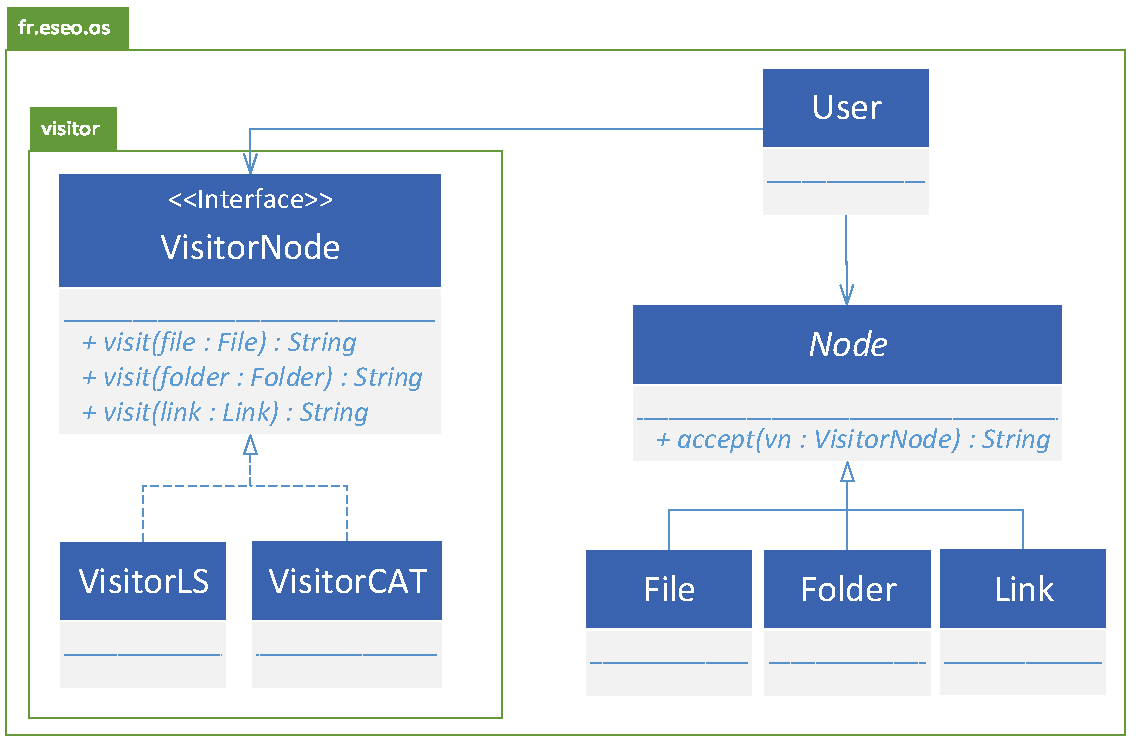
\includegraphics[width=\textwidth]{../uml/uml-visitor}
\end{figure}	

Pour commencer, on a créé une interface \emph{VisitorNode} ayant les méthodes \emph{visit()} pour chaque élément de notre structure (File, Folder et Link) et retournant un résultat.

\begin{lstlisting}
package fr.eseo.os.visitor;
public interface VisitorNode {
	String visit(File file);
	String visit(Folder folder);
	String visit(Link link);
}
\end{lstlisting}

Ensuite, pour chaque commande, on lui associe une classe \emph{VisitorCommande} qui implémente l'interface \emph{VisitorNode}.

\begin{lstlisting}
public class VisitorCAT implements VisitorNode {
	@Override
	public String visit(File file) {
		return file.getData();
	}

	@Override
	public String visit(Folder folder) {
		return "Command not allowed on a folder.";
	}

	@Override
	public String visit(Link link) {
		return link.getTarget().accept(this);
	}
}
\end{lstlisting}

Chaque élément doit implémenter une méthode d'acceptation de visiteur. Nous avons ajouté la méthode abstraite \emph{accept(Visitor)} à la classe Node. 


\begin{lstlisting}
public abstract class Node {
	public abstract String accept(VisitorNode vn);
}
\end{lstlisting}


Et nous avons implémenté cette méthode dans chaque élément de notre structure comme suit :

\begin{lstlisting}
@Override
public String accept(VisitorNode vn) {
	return vn.visit(this);
}
\end{lstlisting}

Enfin, dans la classe \emph{User}, nous avons modifié les méthodes d'appels des commandes comme suit :

\begin{lstlisting}
public String executeCommandLS(String... args) {
    VisitorNode vn = new VisitorLS();
	if (args.length > 1) {
		Node node = this.getHomeDir().findNode(args[1]);
		if (node == null) {
            result =  args[1] + " not found.";
        } else {
            result = node.accept(vn);
        }
	} else {
		result = this.getHomeDir().accept(vn);
	}
	return result;
}
\end{lstlisting}
